\section{Incidence Geometry in Planes and Spaces}

% Problem 1
\begin{problem}
  Consider the system $[S, \mathscr{L}, \mathscr{P}]$, where $S$ contains exactly four points $A, B, C,$ and $D$, the lines are the sets with exactly two points, and the planes are the sets with exactly three points.
  This "space" is illustrated by the following figure:

  \begin{figure}[!h]
    \centering
    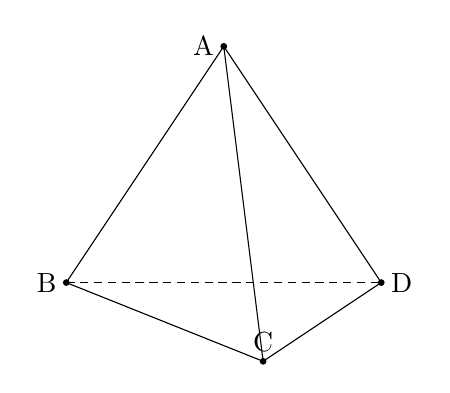
\begin{tikzpicture}[scale = 0.5]
      \draw (0,6) -- (4,0);
      \draw (4,0) -- (1,-2);
      \draw (1,-2) -- (-4,0);
      \draw (-4,0) -- (0,6);
      \draw (0,6) -- (1,-2);
      \draw[densely dashed] (-4, 0) -- (4, 0);
      \filldraw (0,6) circle (2pt) node[anchor=east]{A};
      \filldraw (-4,0) circle (2pt) node[anchor=east]{B};
      \filldraw (1,-2) circle (2pt) node[anchor=south]{C};
      \filldraw (4,0) circle (2pt) node[anchor=west]{D};
    \end{tikzpicture}
    \renewcommand{\thefigure}{2.5}
    \caption{}
  \end{figure}

  Here it should be remembered that $A, B, C,$ and $D$ are the only points that count.
  Verify that all the incidence postulates hold in this system.
\end{problem}

\begin{solution}
  \begin{itemize}
    \item Postulate 1-0 is clearly satisfied by our definitions of the sets $\mathscr{L}$ and $\mathscr{P}$.
    \item Postulate 1-1 is also trivially true by our definition of the set $\mathscr{L}$.
    \item Postulate 1-2 hold since by our definition of lines there are no three collinear points.
      Thus by definition of $\mathscr{P}$ this postulate holds.
    \item Postulate 1-4 is true since there are only four planes in this space, it is easy to check that for any two of them their intersection will be a line.
    \item Postulate 1-5 trivially holds by our definitions of the sets $S, \mathscr{L},$ and $\mathscr{P}$.
  \end{itemize}
\end{solution}

% Problem 2
\begin{problem}
  Let $P_1, P_2, \ldots, P_5$ be five points, no three of which are collinear.
  How many lines contain two of these five points?
\end{problem}

\begin{solution}
  For any two points we select it is clear that the line containing them is unique by Postulate 1-1 and that no other line passing through some other two points is the same line, as there are no collinear points.
  Thus the amount of lines we have is simply $\binom{5}{2} = \frac{5 \cdot 4}{2} = 10$.
\end{solution}

% Problem 3
\begin{problem}
  If no four of the five points are coplanar, how many planes contain three of the five points.
\end{problem}

\begin{solution}
  Similarly to above, any three points we choose define a new, unique plane.
  Thus we know that the amount of planes is $\binom{5}{3} = \frac{5 \cdot 4 \cdot 3}{3 \cdot 2} = 10$.
\end{solution}

% Problem 4
\begin{problem}
  Given $P_1, P_2, \ldots, P_n,$ all different, such that no three of them are collinear and no four of them are coplanar.
  How many lines contain two of them?
  How many planes contain three of them?
\end{problem}

\begin{solution}
  From the same reasoning as above we have $|\mathscr{L}| = \binom{n}{2} = \frac{n (n - 1)}{2}$ and $|\mathscr{P}| = \binom{n}{3} = \frac{n (n - 1) (n - 2)}{3!}$.
\end{solution}

% Problem 5
\begin{problem}
  Show that under our incidence postulates, $S$ cannot be a line.
\end{problem}

\begin{solution}
  Postulate 1-5 requires $S$ to contain at least four noncollinear points.
  However if $S$ was a line, then all points of $S$ are collinear by definition, a contradiction.
\end{solution}

% Problem 6
\begin{problem}
  Show that there is at least one plane.
\end{problem}

\begin{solution}
  By Postulate 1-5 we know that $S$ contains at least four noncollinear points.
  By Postulate 1-2 we know that there exists a plane containing any three different noncollinear points.
  Thus there must be at least four planes.
\end{solution}

% Problem 7
\begin{problem}
  Show that there are at least two planes.
\end{problem}

\begin{problem}
  Follows trivially from the above argument.
\end{problem}
